\documentclass[11pt,a4paper]{article}

%\usepackage[SlantFont]{xeCJK}
%\setCJKmainfont{Hiragino Mincho Pro}
%\setCJKfamilyfont{tt}{Hiragino Mincho Pro}
%\setmainfont[Mapping=tex-text]{Times}
%\usepackage{hyperref}

\usepackage{tgtermes}
\usepackage{tgadventor}
\usepackage[left=28mm,right=28mm,top=30mm,bottom=30mm]{geometry}
\def\baselinestretch{1.1}

\usepackage{graphicx}
\usepackage[colorlinks,unicode]{hyperref}
%\usepackage[whole]{bxcjkjatype} 
%\usepackage{ulem}
\usepackage{amsmath}
\usepackage{amssymb}
\usepackage{braket}

\def\alert#1{\textbf{\textcolor{red}{\uwave{#1}}}}
\def\bC{\mathbb{C}}
\def\bR{\mathbb{R}}
\def\bZ{\mathbb{Z}}

\begin{document}
\centerline{\Large\bfseries Term-end projects for ``Algebraic topology for physicists''}

\bigskip

\centerline{for the autumn-inter semester, academic year 2024 }

\hbox{}\hfill Last update: Dec.~18, 2024

\bigskip

Please answer \emph{at least one} of the questions below,
write it as a term-end paper,
and upload it to the UTokyo LMS page of this lecture series. 
I haven't decided the deadline yet, but it is probably around the last week of January.

\section{Hopf fibration}

We discussed the Hopf fibration $S^1\to S^3\to S^2$. 
$S^3$ can be projected to $\bR^3$ using a stereographic projection.
Objects in $\bR^3$ can then be further projected to a computer screen and or drawn on a paper.

\begin{itemize}
\item Visualize the Hopf fibration itself, for example by drawing the inverse images of various points on $S^2$.
If you create an animation or an interactive program, please upload it online and provide a link to it in the term-end paper.
\item (Optional) 
We also discussed the construction of the connecting homomorphism $\partial : \pi_2(S^2)\to \pi_1(S^1)$ associated to the Hopf fibration.
Visualize this in a way which satisfies you.
\end{itemize}

\section{Topological solitons, 1}

By now there are tons of papers about experimental observations of topological solitons.
Pick (at least) one paper and give a summary, again to your heart's content.

\section{Topological solitons, 2}

The order parameter of superfluid Helium-3 is a homogeneous space $G/H_A$ or $G/H_B$, where 
\begin{itemize}
\item $G=SO(3)\times SO(3)\times U(1)$ , and
\item $H_A$ and $H_B$ are subgroups depending on whether we are in the superfluid A-phase or the B-phase,
\end{itemize}
as described during the lectures and in the lecture note. 

Compute their homotopy groups $\pi_1$ and $\pi_2$. 
It is of course OK to refer to various textbooks, or original papers!


\section{Alternative ``derivation'' of the Dirac quantization law}

We discussed the Dirac quantization law from a rather mathematical perspective.
It is known that the same condition can be derived from the following consideration.
Put an electrically charged particle of charge $e$ at $p=(-1,0,0)$,
and a magnetic monopole of charge $m$ at $q=(+1,0,0)$.
The pattern of the electric field and the magnetic field creates a nonzero Poynting vector,
as seen below: \[
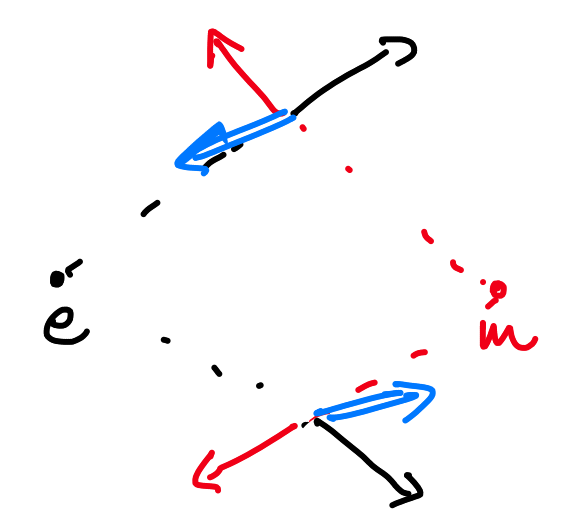
\includegraphics[width=.3\textwidth]{dq.png}
\]
This creates an angular momentum around the axis connecting the points $p$ and $q$.
Demand that it equals the minimal allowed value $\hbar/2$ in quantum mechanics.
What do you find as the magnetic charge $m$ of the magnetic monopole?

(Optional) The derivation here is very different from the one given during the lectures.
Are there any relation?

\section{Kitaev's toric code and cohomology groups}

During the lectures and in the lecture notes, we discussed how Kitaev's toric code 
gives a Hamiltonian whose ground state has basis states
labeled by elements of $H^1(M;\bZ_2)$ as realized by simplicial or cellular cohomology groups.

\begin{itemize}
\item Generalize this to $H^1(M;A)$ for an arbitrary finite Abelian group $A$.
\item (Optional) generalize this to $H^p(M;\bZ_2)$ for a higher $p$.
\item (Optional) generalize this to $H^p(M;A)$ for a higher $p$ and an arbitrary finite Abelian $A$.
\end{itemize}

\section{Some computation of (co)homology groups, 1}

Let $\Sigma_g$ be an oriented compact two-dimensional surface of genus $g$.
Give it a simplicial or cellular decomposition,
and compute $H_p(\Sigma_g;\bZ)$ and $H^p(\Sigma_g;\bZ)$.

(Optional) How about the same question for non-orientable surfaces?

\section{Some computation of (co)homology groups, 2}

Realize $S^{2n-1}$ as the unit sphere in $\bC^n$, parameterized by $(z_1,\ldots,z_n)$.
Let $\bZ_k$ act on it via 
\[
(z_1,\ldots,z_n)\mapsto e^{2\pi i/k} (z_1,\ldots, z_n).
\]
We have a quotient $M=S^{2n-1}/\bZ_k$.
Compute its homology groups $H_p(M;\bZ)$ and $H^p(M;\bZ)$.

Hint: the cell decomposition and much more is explained in Hatcher's textbook, Example 2.43.

\section{$U(1)$ bundles with zero $[F]$ and nonzero $c_1$}

In the exercise above, you find that $H^2(M;\bZ)=\bZ_k$ for $M=S^{2n-1}/\bZ_k$.
This means that it is possible to have  a $U(1)$ bundle $P$ over it such that
 its first Chern class $c_1(P)$ is the generator $1$ of this $\bZ_k$.
As $k\cdot 1=0\in \bZ_k$, $kc_1(P)=0$. 
Correspondingly, $k[F]=0$ in the de Rham cohomology class,
but this simply means that $[F]=0$.
This means that the curvature \emph{does not} contain all the information of the first Chern class.

Let us study a systematic construction of such $U(1)$ bundles.
We first consider a trivial $U(1)$ bundle over $S^{2n-1}$, parameterized by \[
(z_1,\ldots,z_n;w)
\] where $w\in \bC$ parameterizes the fiber. 
We put a trivial connection, whose  curvature is also trivial $F=0$.
We now let $\bZ^k$ to act also on the fiber: \[
(z_1,\ldots,z_n;w)\mapsto e^{2\pi i/k} (z_1,\ldots, z_n;w).
\]
Compute $c_1$ of this bundle  following the steps described below.
\begin{itemize}
\item Argue that this line bundle comes from a $\bZ_k$ bundle over $M$.
As discussed in the lectures, it determines an element in $a\in H^1(M;\bZ_k)$.
\item Using a fine enough cover and the definition of $c_1(P)$ in the lecture notes, 
show that  \[
c_1(P)=\beta(a)\in H^2(M;\bZ)
\]
where $\beta$ is the Bockstein associated to $0\to\bZ \xrightarrow{\times k}\to \bZ\to \bZ_k\to 0$.
(Hint: in the lecture notes we used the sequence $0\to\bZ\to \bR\to U(1)\to 0$ instead.)
\item 
Now that we established the formula above, we can compute the Bockstein in the cellular cohomology,
not in the \v Cech cohomology.
Compute $a$ and $\beta(a)$ using a cell decomposition of $M=S^{2n-1}/\bZ_k$,
and show that $\beta(a)$ is indeed $1\in \bZ_k$.
\end{itemize}

\section{Density matrices vs.~wavefunctions for $n$-level systems}

In the lectures, we learned how to decide when a family 
of $2\times 2$ density matrices over some parameter space $M$
can be lifted to a family of qubits, i.e.~a complex vector bundle $\bC^2\to E\to M$.

\begin{itemize}
\item Generalize the discussion there to  $n$-level systems. That is,
discuss when a family of $n\times n$ density matrices over $M$
can be lifted to a family of $n$-dimensional Hilbert spaces $\bC^n\to E\to M$.
Describe the characteristic class obstructing  this.
\item Discuss an example of a family of $n\times n$ density matrices  over $M$ for $n=3$,
which cannot be lifted to a family of three-dimensional Hilbert spaces.
\end{itemize}

\end{document}